\section{Introduction}

Give a child a 3D model of a pot and a box of bricks, and the question is not whether the pot can be approximated but
how well it can be approximated with the bricks at hand. This paper is about that question for a computer: given a
3D shape and a limit on the number of bricks, produce a model that (a) looks like the shape, (b) is physically legal,
in that every brick sits on studs and nothing overlaps, (c) holds together as a single structure, and (d) comes with
an assembly order a person can follow. Figure~\ref{fig:teaser} shows the task on one mesh.

\begin{figure}[t]
  \centering
  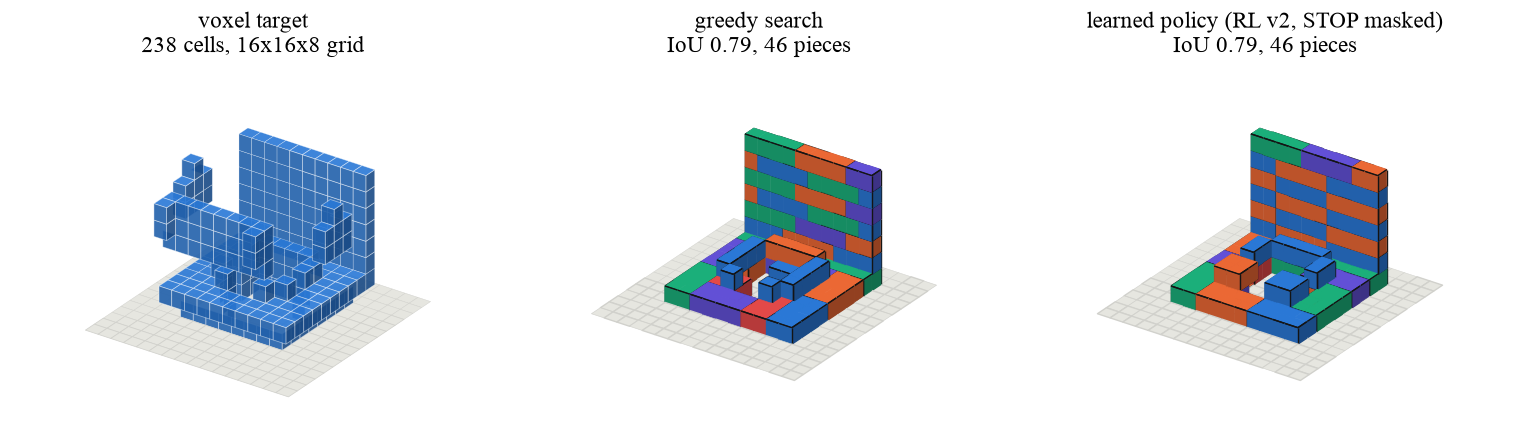
\includegraphics[width=\linewidth]{teaser}
  \caption{The task. A Thingi10K mesh is voxelized onto a 16\,$\times$\,16\,$\times$\,8 grid (left) and rebuilt from
  six kinds of brick under a 200-piece budget by the hand-written greedy search (middle) and by the learned policy
  after reinforcement learning (right). Both builds pass the same validator and assembly planner. Brick colours are
  only there to separate neighbouring pieces.}
  \label{fig:teaser}
\end{figure}

The problem is interesting because it is \emph{discrete} and \emph{constrained}. Each decision is a choice among
hundreds of legal placements, a wrong choice can block a cell forever, and whether the final structure is one
connected piece or several loose islands only becomes clear at the end. Classical approaches search this space with
hand-written heuristics. A natural question is whether a small learned policy can do as well, and whether the extra
signal available from the finished build (its fidelity, its connectedness) can be used to train that policy beyond
imitation. A second, practical question is how fidelity depends on the piece budget: a 50-piece model is cheaper to
buy and faster to build than a 200-piece one, and a designer needs to know what is lost.

We answer both questions inside one controlled pipeline. The pipeline fixes the grid (16 studs by 16 studs by 8 brick
layers), the catalogue (six basic bricks), the legality rules, the trim that keeps the largest ground-connected
component, the assembly planner, the validator and a simplified static stability check. Three generators are swapped
in and out of that pipeline:
\begin{itemize}
  \item a \textbf{greedy search} that tiles each layer bottom-up, covering the most constrained cells first;
  \item a \textbf{learned policy}, a 3D convolutional network with about 100k parameters that scores every legal
  placement plus a stop action, trained by \emph{supervised fine-tuning} (SFT) to imitate the search;
  \item the same policy after \textbf{reinforcement learning} (RL) with proximal policy optimisation (PPO), rewarded
  only by the fidelity and model-stability of the finished, trimmed build.
\end{itemize}
Everything is evaluated on a frozen benchmark of 53 held-out cases (13 procedural shapes and 40 Creative Commons
meshes from Thingi10K) at budgets of 50, 100 and 200 pieces, with an audit that regenerates every recorded number.

\paragraph{Findings.} At the 200-piece cap the RL policy with its stop action masked scores a mean intersection-over-union
(IoU) of \meanRlVTwoNostopTwoHundred{} against \meanGreedyVOneTwoHundred{} for the search; it ties the search on procedural shapes
(\meanRlVTwoNostopProc{} vs \meanGreedyVOneProc{}), trails it by 0.015 on real meshes, matches its validity (\validRlVTwoNostop/53) and
model-stability (\stableRlVTwoNostop/53) counts, and decodes in about twice the search's time, both under 0.2\,s per shape.
Its head-to-head record against the search (wins / losses / ties) is \hhRlVTwoNostopVsGreedyVOne; the median case is a tie
and the gap sits in a handful of real meshes. A second training seed reproduces the number exactly. Each stage of the ladder earned its
place: rebalancing the training data towards real meshes moved SFT from \meanSftVOneTwoHundred{} to \famSftVTwoTwoHundred{} (two-seed mean),
RL on top added between 0.02 and 0.04 over its own initialisation in both seeds, and masking the stop action
added another 0.02 to 0.03. Fidelity rises steeply from 50 to 100 pieces and barely from 100 to 200, for every
generator, because the greedy and the policy both stop when no supported placement remains rather than at the cap.

\paragraph{What did not work.} We report three negative results. The learned stop action remains miscalibrated on
real meshes after RL: with its own stop the policy ends some builds at zero pieces, and masking the action gains 0.03
to 0.09 IoU on a held-out split. The stability bonus in the reward turned out to be redundant: without it the builds
are exactly as stable (under the model) because the legality rules and the trim already enforce what the bonus
rewards. And the connectivity inputs added for RL help wherever the policy has to judge on its own (its own stop
decision, the larger held-out split) but are invisible in the benchmark mean once stop is masked and the trim cleans
up after decoding.

\paragraph{Contributions.}
\begin{enumerate}
  \item A reproducible, audited piece-budget benchmark for brick building with full failure accounting (every case
  reported, failed builds scored zero).
  \item A controlled ladder, greedy $\rightarrow$ SFT $\rightarrow$ SFT+RL on two datasets and two seeds, that
  isolates the effects of data, reinforcement learning and the decode rule.
  \item Evidence that a 100k-parameter candidate-scoring policy trained in under five hours on a laptop reaches within
  0.012 mean IoU of a hand-engineered search at comparable decode cost.
  \item Three negative results about stop calibration, reward shaping and input features, each with the evidence that
  would have been needed to claim the opposite.
\end{enumerate}
